\chapter{Neue Features}
\section{Neuerungen am Server}

\subsection{Web-Crawler}

Eine wichtige Komponente in einer Suchmaschine ist der Crawler, welcher die zu indexierenden Dokumente herunterl�dt. Die bisherige recht einfache Implementierung hat diesen Job nur teilweise gut erledigt. So war es bisher nicht m�glich die Codierung der heruntergeladenen Daten korrekt zu bestimmen. Au�erdem konnte Teamfound nicht mit Framesets umgehen, bzw. hat versucht die Datei mit dem Frameset zu indexieren, nicht den Inhalt der eigentlichen Frames.
 
Um diese Probleme zu l�sen wurde der Teamfound-Crawler komplett neu implementiert. Eine dreistufige Suche nach einer Codierungsangabe, n�mlich in der Verbindung an sich, im HTTP-Header sowie im HTML-Header. Letzterer Ort ist der warscheinlichste Fundort f�r ein solches Encoding. Es ist daf�r also notwendig den kompletten HTML-Code herunterzuladen und dann nach einer entsprechenden Angabe zu suchen. Die Suche nach Angaben zum Encoding sieht die M�glichkeit vor, das Teamfound in der Zukunft mehrere Arten von Dokumenten indexieren kann. Da die Suche nach einem Encoding in PDF-Dateien zB. ganz anders ablaufen wird, muss diese vom Inhaltstyp abh�ngen. Der neue Crawler l�sst sich bequem um solche erweitern.

Die Behandlung von Framesets ist eine zentrale Anforderung, die auf verschiedene Arten gel�st werden kann. So ist die Frage, ob einfach alle Frames in der Reihenfolge ihrer Definition in der Quelldatei heruntergeladen und zu einem langen Dokument zusammengef�gt werden, oder ob mehr Aufwand betrieben werden soll, um zB. den Hauptinhaltsframe zu finden und an den Anfang des Ergebnisdokumentes zu stellen. Die neue Implementierung des Crawler verfolgt erstes Schema, alle Frames werden in einfacher Definitionsreihenfolge hintereinander kopiert und dann an den Indexer �bergeben, welcher das HTML entfernt und den Text indexiert. So steht aber nat�rlich nicht immer der Anfang des Inhaltes in der Teamfound-Ergebnisanzeige. Da es aber nicht einfach ist, den Hauptinhaltsframe innerhalb eines Framesets herauszufinden haben wir uns entschieden dieses auch nicht zu versuchen.

\subsection{Index-Updates}

Wurden bisher Internetseiten in einen Teamfound-Server aufgenommen so wurden sie w�hrend dieses Vorganges vom Crawler heruntergeladen und in den Index gespeichert. �nderungen an der Seite w�rden sp�ter nicht in den Index aufgenommen werden da bereits eingetragene Seiten nicht erneuert wurden.
Um dieses Problem aus der Welt zu schaffen startet ein Teamfound-Server nun einen nebenl�ufigen Thread der alle Seiten in einem bestimmten Intervall erneut herunterl�dt und bei �nderungen neu indexiert.

Dabei k�nnen Seiten, wenn der Crawler auf HTTP-Fehler st��t, vorr�bergehend deaktiviert werden, oder wenn diese Fehler anhalten, auch komplett aus dem Index entfernt werden.

\subsection{Logging}

Da der Funktionsumfang des Teamfound-Servers stark angewachsen ist, wurde die Nutzung eines echten Logging-Systems notwendig, einerseits vereinfacht dies die Entwicklung, da Debug-Ausgaben ordentlich ausgegeben werden k�nnen, andererseits ist es f�r einen sp�teren Produktiven Einsatz evtl. wichtig Fehler bei Zugriffen auf den Teamfound-Server oder fehlgeschlagene Logins zu protokollieren.
Da w�hrend eines produktiven Einsatzes keine oder nur wenige Debug-Nachrichten protokolliert werden sollen, ist ein Logging-System notwendig, das einerseits zwischen der Art von Nachrichten unterscheiden kann, andererseits aber auch Komponenten, welche Nachrichten einliefern, trennen kann. log4j aus dem Apache-Projekt erf�llt alle diese Aufgaben und wurde daher f�r die Integration in Teamfound ausgew�hlt. Einzelne Komponenten benutzen unterschiedliche sogenannte 'Logger' und trennen ihre Nachrichten in mehrere Kategorien zwischen Debug, Info sowie Warning und Error auf. Einzelne oder alle Logger k�nnen auf die Konsole oder in eine Datei umgeleitet werden.  

\subsection{Usermanagement}

Mit Einf"uhrung eines Usermanagements wurden viele Erweiterungen an unterschiedlichen Stellen im Server notwendig.
Die Datenbank muss erweitert werden, neue Aufrufe m"ussen im Servlet entgegengenommen und
dann im Server ausgef"uhrt werden. Ausserdem muss bei alter sowie neuer Funktionalit"at eine "Uberpr"ufung der Berechtigung durchgef"uhrt werden.
Um vern"unftige Nutzbarkeit zu erreichen ist zus"atzlich ein Sessionmanagement n"otig.

Da vom ServletContainer ein Mechanismus f"ur Sessions angeboten wird, war hier haupts"achlich zu kl"aren welche Informationen zu jeder Session gehalten werden und wie diese organisiert sind.

Die neuen Informationen, die in der Datenbank zu speichern sind, waren ziemlich klar, deshalb konnte 
die Grundlage ziemlich schnell geschaffen werden ohne das sp"ater gr"ossere "Anderungen n"otig
wurden.
Die interne Programmlogik war wohl am aufwendigsten. Der wachsende Funktionsumfang und
die n"otige Authorisierungpr"ufung ergeben deutlich komplexere Vorg"ange als in der
vorhergehenden Version zu Milestone 2.


Neue Funktionalit"at des Servers :
\begin{itemize}
\item 3 Benutzertypen : Projektadmin , angemeldeter Nutzer, anonymer Nutzer
\item Zuordnung von Nutzern/Admins zu Projekten
\item Berechtigungsvergabe auf Projektebene
\item L"oschen von Kategorien und indizierten Dokumenten durch berechtigte Nutzer
\end{itemize}

\subsection{Server Einstellungen}
Bei wachsender Funktionalit"at des Servers wird auch eine vern"unftige Ausgangkonfiguration 
notwendig. Daf"ur existiert ein Konfigurationsfile, welches "uber den von Java angebotenen
Properties Mechanismus eingelesen und verwendet wird.


Derzeit sind folgende Werte einstellbar :
\begin{itemize}
\item Der Pfad, in welchem die Datenbank und der Index angelegt werden sollen 
\item Ein initiales Projekt
\item Ein User, der auch Admin zum Projekt sowie Systemadmin ist
\item Die Tiefe in der Framesets aufgel"ost werden sollen
\item Das Maximalalter, welches eine Dokument haben darf, bevor es vom Updater erneuert wird (in Tagen)
\item Die Zeit in Minuten, die der Updatethread schlafen soll bevor er die n"achste Aktion ausf"uhrt
\end{itemize}


\section{Neuerungen am Web-Interface}
\begin{figure}
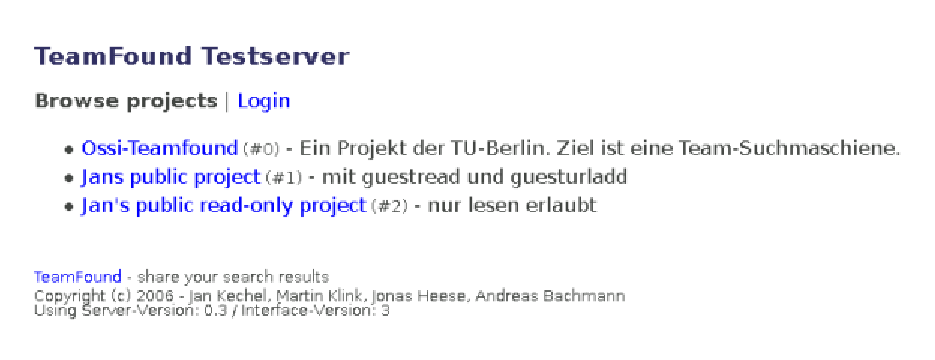
\includegraphics{web1.eps}
\caption{Web-Interface Eingangsseite}
\end{figure}

\textit{Neuerungen} ist gut, bisher gab es eigentlich noch kein Web-Interface :)

Die Version 0.2 des TeamFound Servers hatte noch die Option \texttt{want=xml|html}, "uber die man vom Server direkt eine im Browser darstellbare HTML-Seite anfordern konnte. Jedoch war dieser Teil des Servers zu grossen Teilen nicht implementiert.

In der aktuellen Version 0.3 setzen wir nur auf XML-Antworten, die daf"ur aber allesamt ein XSL-Transformations Stylesheet enthalten:

\texttt{<?xml-stylesheet href=$``$transform.xsl$``$ type=$``$text/xsl$``$?>}

"Uber diese XSLT Datei k"onnen alle g"angigen Browser das vom Server gelieferte XML selber in HTML umwandeln und anzeigen.

\begin{figure}
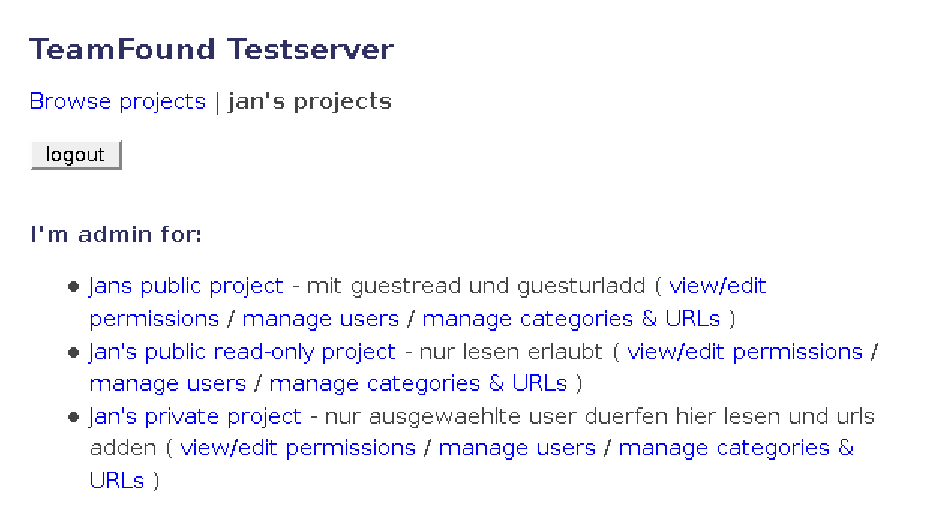
\includegraphics{web2.eps}
\caption{Web-Interface "Ubersicht der eigenen Projekte}
\end{figure}


\subsection{Komponenten}
Das gesamte Web-Interface besteht aus 3 Dateien:
\begin{description}
\item[transform.xsl] Transformiert unseren XML-Baum in HTML.
\item[stylesheet.css] Legt das Layout des erstellten HTMLs fest.
\item[ui.js] Enth"alt eine einzige JavaScript Funktion (\texttt{showhide(layer\_ref)}) zum Anzeigen/Verstecken einzelner Bereiche der Webseite.
\end{description}

Die \texttt{transform.xsl} ist die einzige dieser Dateien die ich hier genauer beschreiben will. Sie besteht, wie jede XSLT Datei aus verschiedenen Templates, die jeweils bestimmte XML Unterb"aume in HTML umwandeln. Als erstes kommt das template \texttt{match=/response} zum Tragen, da unsere XML-B"aume alle von dem tag \texttt{response} umschlossen werden. Es erstellt zuerst die allgemeinen HTML-Header, ruft dann der Reihe nach die 3 templates \texttt{menu}, \texttt{showcommandresults} und \texttt{pageselector} auf, und beendet seine Arbeit mit dem Ende der HTML-Seite incl. einem Link zur teamfound Webseite und einem Copyright Hinweis.

\begin{description}
\item[menu] Erzeugt nur das Men"u der Seite entsprechend dem Parameter \texttt{xsltpassthrough}. 
\item[showcommandresults] Durchsucht den XML-Baum nach den verschiedenen Antworten der m"oglichen Befehle und zeigt die Ergebnisse entsprechend an. 
\item[pageselector] Ruft entsprechend den \texttt{xsltpassthrough}-Parametern spezialisierte templates auf, die jeweils Seiten f"ur die Bedienung der verschiedene Server-Befehle mittels HTML-Formularen erzeugen. 
\end{description}

\begin{figure}
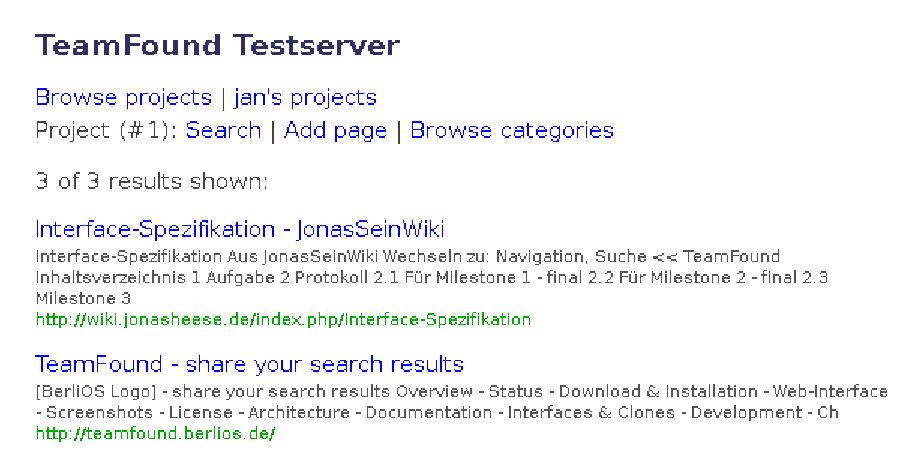
\includegraphics{web3.eps}
\caption{Web-Interface Suchergebnisse und Projekt-Menu}
\end{figure}

Unterst"utzt werden alle im Interface Milestone 3 festgelegten Befehle. Den genauen Aufbau der Webseite schaut sich am besten jeder selber auf unserem Testserver \texttt{http://teamfound.dyndns.org:8080/tf/tf} an.

\section{Firefox/Flock-Toolbar}
Nichts besonderes. Die Toolbar wurde nur an das Interface Milestone 3 angepasst. Die Projektverwaltung und Administration wird nicht unterst"utzt, sondern hier verweise ich freundlichst auf das Web-Interface :-)

\clearpage
\section{Projekt-Webseite}
Aktualisierte Version, angereichert mit Werbe-Text: 

\texttt{http://teamfound.berlios.de}
\begin{figure}[h]
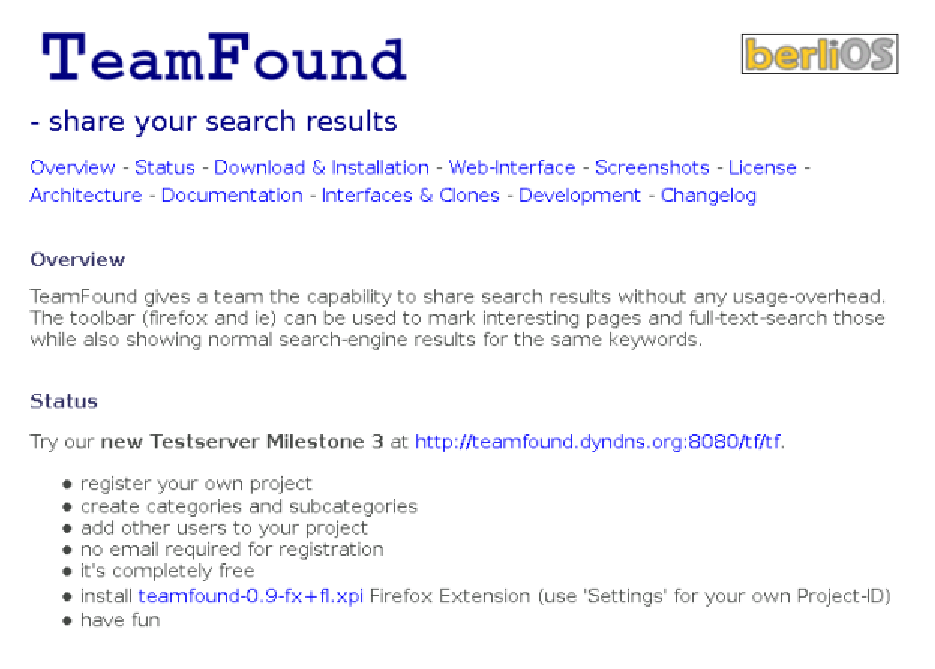
\includegraphics{web4.eps}
\caption{Projekt Webseite}
\end{figure}

\clearpage

\section{Neuerungen an der Internet-Explorer-Toolbar}

Die Arbeiten an der Toolbar teilen sich in zwei Bereiche Anpassungen und Erweiterungen. Die Toolbar besteht aus aus einer Sammlung von Views, der Controller Klasse und einer Menge von Datenklassen (Modell). Durch diese Trennung ist die Erweiterung recht gut m"oglich. Neue Objekte wie Projekte, Benutzer und Berechtigungnen wurden zuerst als Datenobjekte implementiert und die dazugeh"orige Logik der Controller Klasse hinzugef"ugt.
Wo notwendig wurden Views zu Visualisierung erstellt. Es ist abzusehen das mit falls weitere Funktionalit"at hinzugef"ugt wird, ein Teil der Logik aus der Controller Klasse, in Service Klassen ausgelagert werden muss. 

Ansonsten habe ich mit der Verwendung eines Testprogramms begonnen. Der Ansatz verdeutlicht das es m"oglich ist die Funktionen der Toolbar auch ausserhalb des Internet Explorers zu nutzen. Somit k"onnte auch eine Integration in Entwicklungsumgebungen stattfinden (z.B. Visual Studio).

\subsection{Anpassungen}

Es war vollen allem notwendig die Suche so anzupassen das Sie mit den "Anderungen aus Milestone 3 klar komment. Als erstes w"aren da die neu eingef"uhrten Projekte zu nennen. Da ein Projekte eine Kategorie ist, "andert sich an der Suche direkt nichts. Es ergibt sich jedoch die Notwendigkeit eine M"oglich f"ur die Projektauswahl und die Kategorienauswahl in Abh"angikeit davon zu gestalten. 

Weiterhin musste die neue Dokumentstruktur unterst"utzt werden. Da die Toolbar die Sucherergebnisse intern als Objekte verwaltet war der Aufwand in der Anpassung nicht so gro�.

\subsection{Erweiterungen}

Wie bereits im Ablauf beschrieben, wurde der bisherige Einstellungsdialog ersetzt. Statt nur eine einzelne Serveraddresse eingeben zu k"onnen, hat der User nun die M"oglichkeit diverse Server zu verwalten. Zu jedem Server k"onnen jetzt Addresse, Benutzer und Passwort, die Projekte, deren Benutzer und die jeweiligen Kategorien und Berechtigungen verwaltet werden. Im wesentlichen entspricht die Funktionalit"at der des Web Interface. 


